6. Для нахождения области определения $f(x)$ необходимо решить неравенство\\ $\cfrac{-x(x^2-2x-15)(x^2-6x+8)}{(x^2-11x+30)(x+1)}\geqslant0
\Leftrightarrow \cfrac{-x(x-5)(x+3)(x-2)(x-4)}{(x-5)(x+6)(x+1)}\geqslant0.$ Решим его, применив метод интервалов:
$x\in[-3;-1)\cup[0;2]\cup[4;5)\cup(5;6).$
\begin{figure}[ht!]
\center{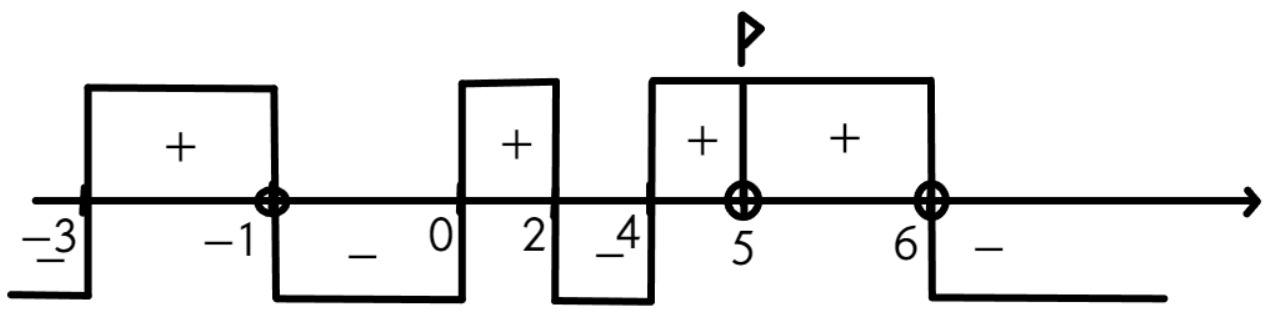
\includegraphics[scale=0.35]{isl9-6.png}}
\end{figure}\\
